\documentclass[xcolor={dvipsnames}]{beamer}
\usepackage{color, colortbl}
\usepackage[ngerman,english]{babel}
\usepackage[T1]{fontenc}
\usepackage{lmodern}
\usepackage[compatibility=false]{caption}
\usepackage{subcaption}
\usepackage{tikz}
\usepackage{textgreek}
\usepackage{tabularx}
\usepackage{booktabs}
\usepackage{xspace,multicol}
\usepackage{siunitx}
\usepackage{appendixnumberbeamer}
\usepackage[absolute,overlay]{textpos} %for positioning the logos where I want


\usepackage{animate}
\usepackage{multimedia}
\usepackage{fixltx2e}
\usepackage{multicol}
\usepackage{multirow}
\usepackage{comment}
\DeclareSIUnit\year{yr}
\DeclareSIUnit\micron{\micro\metre}
\DeclareSIUnit\mrad{\milli\rad}
\DeclareSIUnit\gauss{G}
\DeclareSIUnit\nb{\nano\barn}
\DeclareSIUnit\pb{\pico\barn}
\DeclareSIUnit\fb{\femto\barn}

\newcommand{\electron}{e$^-$\xspace}
\newcommand{\positron}{e$^+$\xspace}
\newcommand{\murm}{%
  \ifmmode
    \mathchoice
        {\hbox{\normalsize\textmu}}
        {\hbox{\normalsize\textmu}}
        {\hbox{\scriptsize\textmu}}
        {\hbox{\tiny\textmu}}%
  \else
    \textmu
  \fi
}

\mode<presentation>
{
  \usetheme{CambridgeUS}     
  \usecolortheme{lily} 
  \definecolor{beamer@violet}{rgb}{0.5,0.3,0.5} % changed this
  \setbeamercolor{structure}{fg=beamer@violet!70!cyan}
  \setbeamercolor{palette primary}{fg=black, bg=gray!30!white!50!cyan!20!}
  \setbeamercolor{palette secondary}{fg=black, bg=gray!30!white!30!cyan!40!}
  \setbeamercolor*{palette tertiary}{bg=gray!20!white!20!cyan!60!}
  
  \setbeamercolor{frametitle}{fg=cyan!60!white!40!,bg=cyan!80!black}
  \setbeamercolor{title}{fg=cyan!80!black}
  \setbeamercolor{normal text}{fg=black,bg=white}
  \setbeamercolor{alerted text}{fg=beamer@violet}
  \setbeamercolor{example text}{fg=beamer@violet!70!cyan}
  
  \usefonttheme{structureitalicserif} 
  \setbeamertemplate{navigation symbols}{}
  \setbeamertemplate{caption}[numbered]
}
\newcommand{\sidlogo}{
  \setlength{\TPHorizModule}{1pt}
  \setlength{\TPVertModule}{1pt}
   % textblock{}{x,y}: pos(x) = rightUpperCorner + (x * \TPHorizModule), pos(y) = leftUpperCorner - (y * \TPVertModule)
  \begin{textblock}{1}(323,12)
   \includegraphics[width=40pt,height=26pt]{figures/SiD.jpeg}
  \end{textblock}
  } 
\newcommand{\ilclogo}{
  \setlength{\TPHorizModule}{1pt}
  \setlength{\TPVertModule}{1pt}
   % textblock{}{x,y}: pos(x) = rightUpperCorner + (x * \TPHorizModule), pos(y) = leftUpperCorner - (y * \TPVertModule)
  \begin{textblock}{1}(323,12)
   \includegraphics[width=40pt,height=26pt]{figures/ILC.jpeg}
  \end{textblock}
} 
\newcommand{\flukalogo}{
  \setlength{\TPHorizModule}{1pt}
  \setlength{\TPVertModule}{1pt}
   % textblock{}{x,y}: pos(x) = rightUpperCorner + (x * \TPHorizModule), pos(y) = leftUpperCorner - (y * \TPVertModule)
  \begin{textblock}{1}(315,12)
   \includegraphics[width=60pt,height=26pt]{figures/fluka_logo.png}
  \end{textblock}
} 

\title[ILC backgrounds \& SiD Occupancy]{\textbf{\alert{SiD Optimization Meeting} \\ \vspace*{0.3cm} \LARGE  Update \& summary of BDS muon occupancy studies}}
\author{\textbf{Anne Sch\"utz}}
\institute{\textbf{DESY}}
\date{\textbf{07. March 2018}}

\titlegraphic{\includegraphics[height=1.0cm]{figures/ILC.jpeg}\hspace*{6cm}~%
   \includegraphics[height=1.2cm]{figures/DESY_Logo.png}
}

\begin{document}

{
\usebackgroundtemplate{
 \tikz\node[opacity=0.1]{\includegraphics[width=\paperwidth]{figures/Iwatecomics.jpg}};
 % \tikz\node[opacity=0.2]{\centering\includegraphics[height=\paperheight]{figures/Iwatecomics.jpg}};
 }
\begin{frame}
  \titlepage
\end{frame}
}
\setcounter{tocdepth}{2}
\begin{frame}{Table of contents}
  \tableofcontents
\end{frame}

%---------------------------------------------------------------------------------------------------------



%----------------------------------------------------------------------------------

\section{Muons from the Beam Delivery System}
\subsection{Motivation}

\begin{frame}{BDS tunnel layout}
\ilclogo
\begin{center}
\includegraphics[height=0.65\textheight]{muons_figures/BDS_electron_tunnel.pdf}
\end{center}
\end{frame}

\begin{frame}{Muon spoiler scenarios}
\ilclogo
There are two shielding scenarios under discussion:
\begin{itemize}
 \item \textbf{5 Spoilers}
 \item \textbf{5 Spoilers + Wall}
\end{itemize}

\begin{columns}[b]
 \begin{column}{0.8\textwidth}
 \flushright
\includegraphics[height=0.67\textheight]{muons_figures/BDS_Tunnel_Spoilers+Wall_edited.png}
\end{column}
 \begin{column}{0.2\textwidth}
 \flushleft
e\textsuperscript{-} beam line
\vspace*{0.55cm}
\end{column}
\end{columns}
\end{frame}

\begin{frame}{5 spoilers}
\ilclogo
\textbf{The spoilers} are designed as follows:
\begin{itemize}
 \item \SI{70}{\centi\meter} radius
 \item \SI{5}{\meter} long
 \item Magnetized iron with a field of $\sim$10-\SI{19}{\kilo\gauss}
 \item 5 locations (from the IP):
 \begin{itemize}
  \item 802.5m
  \item 975.5m
  \item 1145.5m
  \item 1234.5m
  \item 1358.5m
 \end{itemize}

\end{itemize}
\begin{center}

\includegraphics[height=0.3\textheight]{muons_figures/spoilers.png}
\end{center}
\end{frame}

\begin{frame}{5 spoilers + wall}
\ilclogo
\textbf{The iron wall} would completely fill up the tunnel:
\begin{itemize}
 \item \SI{3.3}{\meter} x \SI{5}{\meter}, \SI{5}{\meter} long
 \item Magnetized with a field of $\sim$\SI{16}{kG}
 \item Located $\sim$\SI{400}{\meter} away from the IP
 \item Would cost $\sim$ \$3 million
\end{itemize}
\begin{center}
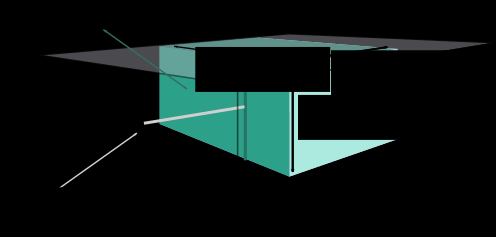
\includegraphics[height=0.4\textheight]{muons_figures/muon_wall.png}
\end{center}
\end{frame}

\AtBeginSubsection[] {
  \begin{frame}<beamer>
     \tableofcontents[currentsection,
     currentsubsection,
     %hideothersubsections,
     subsectionstyle=show/shaded/hide,
     subsubsectionstyle=show/show/hide]
  \end{frame}
}

\subsection{MUCARLO simulation}
\begin{frame}{MUCARLO simulation overview}
\ilclogo

\begin{columns}
 \begin{column}{0.7\textwidth}
  \begin{itemize}
\item BDS backgrounds with muon collimation system modelled with MUCARLO [Lewis Keller, SLAC] and Geant4 [Glen White, SLAC]
\item Using TDR baseline machine parameters for the ILC500 \alert{\& new beam parameters for the ILC250 stage}
\item Muon production processes:
\begin{itemize}
\item Predominantly: Bethe-Heitler process:\\ \textgamma + Z $\rightarrow$ Z' + \textmu$^+$\textmu$^-$
\item Few \% level: direct annihilation of positrons with atomic electrons: e$^+$e$^-$ $\rightarrow$ \textmu$^+$\textmu$^-$
\end{itemize}
\item Halo particle tracking:
\begin{itemize}
\item Turtle with MUCARLO
\item Lucretia with a built-in Geant4 model interface
\end{itemize}
\end{itemize}

 \end{column}
 \begin{column}{0.3\textwidth}
  \includegraphics[width=\textwidth]{muons_figures/BetheHeitler.pdf}
 \end{column}
\end{columns}
\end{frame}

%------------------
\newcolumntype{L}[1]{>{\raggedright\let\newline\\\arraybackslash\hspace{0pt}}m{#1}}
\newcolumntype{C}[1]{>{\centering\let\newline\\\arraybackslash\hspace{0pt}}m{#1}}
\newcolumntype{R}[1]{>{\raggedleft\let\newline\\\arraybackslash\hspace{0pt}}m{#1}}
%-----------------

\subsubsection{Muon 4-vectors}
\begin{frame}{Muons in the detector}
\ilclogo
\centering
\begin{tabular}{ l|C{2.25cm}|C{2.25cm} }
\textbf{Scenario} & \multicolumn{2}{>{\centering}p{5.5cm}}{\textbf{Muons per bunch crossing in a detector with 6.5m radius}}\\
& ILC500 & ILC250\\
\hline\\
 No Spoilers & 130 & 39\\
 5 Spoilers& 4.3 & 1.3\\
 5 Spoilers + Wall & 0.6 &  0.03
\end{tabular}

\end{frame}

\subsubsection{Motivation}
\begin{frame}{}
Do we need the muon wall at all?!
It would be easier without it, because of safety issues, and the costs for such a iron wall.
\begin{center}
\fbox{\includegraphics[height=0.5\textheight]{muons_figures/Muon_wall_required.pdf}}
\end{center}
\textit{On the other hand:}\\
\alert{It serves at a tertiary containment device!\\
Removing the wall would mean NO access to IR when the beam is on!\\
And expecting considerably higher rates when going to 1\,TeV $\rightarrow$ maybe wall then necessary anyway!}
\end{frame}

\section{Results of the Geant4 simulation}
\subsection{Event displays of muons in the SiD detector}
\begin{frame}{WIRED4 event display of muons in SiD}
\sidlogo
Muons from a full bunch train (1312 bunch crossing)\\ \vspace*{0.3cm}
{\small \hspace*{0.2cm} ILC250, spoilers + wall \hspace*{0.7cm} ILC500, spoilers + wall \hspace*{0.7cm} ILC500, spoilers}\\
\includegraphics[height=0.4\textheight]{muons_figures/Event_display_ILC250_p_spoilers_wall.png}\hfill
\includegraphics[height=0.4\textheight]{muons_figures/muons_positron_5spoilers_wall_515_xyview_croped.png}\hfill
\includegraphics[height=0.4\textheight]{muons_figures/muons_positron_5spoilers_2961_xyview_croped.png}
\\\vspace*{0.5cm} The muons exit the BDS tunnel, and penetrate the whole detector.
\end{frame}

\subsection{Analysis - Energy distributions}
\begin{frame}{Energy distribution of muons from a bunch train}
\sidlogo
\begin{center}
  \includegraphics[width=0.75\textwidth]{muons_figures/Energy_Comparison_ILC500vsILC250.pdf}
\end{center}
In the 'Spoiler + Wall' case, the lower energy muons are either stopped or deflected by the magnetized wall.
\end{frame}

%New command: column type
\newcolumntype{P}[1]{>{\centering}p{#1}}

\subsection{Analysis - Total number of hits}
\begin{frame}{Total number of hits for a bunch train}
\sidlogo
\begin{columns}
 \begin{column}{0.23\textwidth}
 \small
  Comparison of the total number of hits in the different SiD subdetectors:
 \end{column}
 \begin{column}{0.8\textwidth}
\includegraphics[width=\textwidth]{muons_figures/Hits_in_SiD_subdetectors_MuonSpoilerStudy.pdf}
 \end{column}
\end{columns}
\begin{center}
\begin{tabular}{@{}p{0.343\textwidth}p{0.01\textwidth}p{0.18\textwidth}p{0.01\textwidth}p{0.343\textwidth}p{0.001\textwidth}@{}}
 \centering Vertex detectors & < & \centering ECAL, HCAL & < & \centering MuonEndcaps & \\
  \centering{\scriptsize Smallest effective detector area} & &  \centering{\scriptsize Particle showers} & &  \centering{\scriptsize Biggest effective detector area}&
\end{tabular}
\end{center}
\end{frame}

\subsection{Analysis - Time distributions}

\begin{frame}{Hit time distribution for a bunch train}
\sidlogo
 \begin{center}
\includegraphics[height=0.75\textheight]{muons_figures/hittime_ILC500_spoilers_superimposed.pdf}
\end{center}
Muons are first hitting the MuonEndcaps as the outermost subdetector.
\end{frame}

\subsection{Analysis - Occupancies}

\begin{frame}{Occupancy plots - \small HcalBarrel}
\sidlogo
{\footnotesize The following occupancy plots are the result of muons from a \alert{full bunch train (1312 bunch crossings)}, and they are normalized by the total number of cells.}\\\vspace*{0.1cm}
\includegraphics[height=0.46\textheight]{muons_figures/Occupancy_Comparison_All_layers_wrt_cells_HcalBarrel.pdf}\hfill
\includegraphics[height=0.46\textheight]{muons_figures/Occupancy_Comparison_All_layers_deadcells_HcalBarrel.pdf}\\
\vspace*{0.2cm}
Only up to three hits per cell $\rightarrow$ Low occupancy
\\'5 Spoilers + Wall' for 250 and 500\,GeV does better by at least one order of magnitude.
\end{frame}

\begin{frame}{Occupancy plots - \small SiTrackerEndcap}
\sidlogo
\includegraphics[height=0.46\textheight]{muons_figures/Occupancy_Comparison_All_layers_wrt_cells_SiTrackerEndcap.pdf}\hfill
\includegraphics[height=0.46\textheight]{muons_figures/Occupancy_Comparison_All_layers_deadcells_SiTrackerEndcap.pdf}\\
Number of hits per cell up to 30 $\rightarrow$ low energy muons spiral, and hit cells several times!
\\For all assumed buffer depth values, the total number of dead cells stays way below 10$^{-4}$ (critical limit).
\end{frame}

\begin{frame}{Occupancy plots - \small All other subdetectors}
\sidlogo
{\footnotesize Tracker Barrel \hspace*{5cm} HCAL Endcap}\\
\includegraphics[height=0.39\textheight]{muons_figures/Occupancy_Comparison_All_layers_deadcells_SiTrackerBarrel.pdf}\hfill
\includegraphics[height=0.39\textheight]{muons_figures/Occupancy_Comparison_All_layers_deadcells_HcalEndcap.pdf}\\
{\footnotesize ECAL Barrel \hspace*{5.2cm} ECAL Endcap}\\
\includegraphics[height=0.39\textheight]{muons_figures/Occupancy_Comparison_All_layers_deadcells_EcalBarrel.pdf}\hfill
\includegraphics[height=0.39\textheight]{muons_figures/Occupancy_Comparison_All_layers_deadcells_EcalEndcap.pdf}\\
\end{frame}
\begin{frame}{Occupancy plots - \small All other subdetectors}
\sidlogo
{\footnotesize Muon Barrel \hspace*{5.2cm} Muon Endcap}\\
\includegraphics[height=0.39\textheight]{muons_figures/Occupancy_Comparison_All_layers_deadcells_MuonBarrel.pdf}\hfill
\includegraphics[height=0.39\textheight]{muons_figures/Occupancy_Comparison_All_layers_deadcells_MuonEndcap.pdf}\\
{\footnotesize BeamCal \hspace*{5.8cm} LumiCal}\\
\includegraphics[height=0.39\textheight]{muons_figures/Occupancy_Comparison_All_layers_deadcells_BeamCal.pdf}\hfill
\includegraphics[height=0.39\textheight]{muons_figures/Occupancy_Comparison_All_layers_deadcells_LumiCal.pdf}\\
\end{frame}


\section{Conclusion}
\begin{frame}
\textit{Updated analysis framework and new numbers for ILC250 have shown:}
\begin{itemize}
 \item Muons penetrate the whole detector horizontally.
 \item At \alert{500\,GeV}, the \alert{5 spoilers} can reduce the number of muons to $\sim$4/bunch crossing, which results in the \alert{highest occupancies}.
 \item The 5 spoilers + wall scenario reduces this significantly.
 \item In the \alert{ILC250 stage}, the number of \alert{muons/bunch crossing is reduced to $\sim$ 1}.
 \item The \alert{occupancies} are for all scenarios \alert{well below $\sim10^{-4}$}.
\end{itemize}
\textit{Conclusion:}
\begin{itemize}
\item High energy muons could be used for tracker alignment.
\item Spatial distributions quite different in scenarios w/ \& w/o the wall.
\item With the shown evaluation of the muons from the current MUCARLO simulations, the \alert{magnetized wall is not required for limiting the detector occupancy in the ILC250 stage}.
However, the wall serves as a tertiary containment device, and might be mandatory anyway.
\item Maybe instead a shielding wall which is not magnetized $\rightarrow$ cost reduction
\end{itemize}
\end{frame}

%---------------------------------------------------------------------------------

\section*{The end}
{
\usebackgroundtemplate{
 \tikz\node[opacity=0.1]{\includegraphics[width=\paperwidth,resolution=200]{figures/ilc-Comic.png}};
 % \tikz\node[opacity=0.2]{\centering\includegraphics[height=\paperheight]{figures/Iwatecomics.jpg}};
 }
\begin{frame}
\ilclogo
\begin{center}
\textcolor{RubineRed}{
	\LARGE Thanks!\\
}
\end{center}
\end{frame}
}

\section*{References}
\begin{thebibliography}{9}
\setbeamertemplate{bibliography item}[text]
\begin{frame}{References for the BDS muon study}
\tiny
\bibitem{MUCARLO_talk}  \emph{ECFA 2016: Talk by Glen White about the MUCARLO simulation of the muons from the muon spoilers}. \url{https://agenda.linearcollider.org/event/7014/contributions/34689/attachments/30076/44961/ILC_muons.pptx}
\bibitem{Jonas_talk}  \emph{DESY summer student program: Talk by Jonas Glomitza (RWTH Aachen) about ``The Impacts of the Muon Spoiler Background on the ILC Detector Performance'', 08. September 2016}. \url{https://indico.desy.de/getFile.py/access?contribId=9&resId=0&materialId=slides&confId=15972}
\bibitem{Suppression}  \emph{FERMILAB-CONF-07-276-AD: ``Suppression of Muon Backgrounds generated in the ILC Beam Delivery System'', Drozhdin et.al, 2007}. \url{https://inspirehep.net/record/771808/files/fermilab-conf-07-276.pdf}
\bibitem{MUCARLO}  \emph{``Calculation of Muon Background in Electron Accelerators using the Monte Carlo Computer Program MUCARLO'', Rokni et.al}. \url{http://www.slac.stanford.edu/cgi-wrap/getdoc/slac-pub-7054.pdf}
\bibitem{MuonBackground_1TeV}  \emph{SLAC-PUB-6385: ``Muon Background in a 1.0-TeV Linear Collider'', L.P. Keller, 1993}. \url{http://www.slac.stanford.edu/pubs/slacpubs/6250/slac-pub-6385.pdf}
\bibitem{MuonBackground_0.5TeV}  \emph{SLAC-PUB-5533: ``Calculation of Muon Background in a 0.5 TeV Linear Collider'', L.P. Keller, 1991}. \url{http://www.slac.stanford.edu/cgi-wrap/getdoc/slac-pub-5533.pdf}
\end{frame}

\end{thebibliography}

%--------------------------------------------------------------------------------
\section{Backup}
\appendix

\begin{frame}
\begin{center}
\LARGE Additional Material
\end{center}
  \tableofcontents
\end{frame}

\section{Prerequisites}
\subsection{Beam halo}
\begin{frame}{Beam halo definition}
Beam core:
\begin{itemize}
 \item an ellipse with a horizontal size of $\pm 5\sigma_x$ and a vertical size of $\pm 36\sigma_y$ at the beginning of the BDS
\end{itemize}
Beam halo:
\begin{itemize}
 \item elliptical ring around the beam core, covering 5-13$\sigma_x$ and 36-93$\sigma_y$
 \item beam particle intensity in the core follows a $\frac{1}{r}$ distribution
 \item beam power of the halo is normalized to \SI{0.1}{\percent} of the nominal beam power
\end{itemize}

\end{frame}

\subsection{Muon sources}
\begin{frame}{BDS collimators as muon sources}
The main sources of muons were identified in the BDS to be 11 distinct collimators.
\begin{itemize}
 \item Primary collimator spoilers (radiation length: 0.6 X\textsubscript{0}, half-gap: \SI{930}{\micro\meter} in x, \SI{400}{\micro\meter} in y):\\
  SP2 (\SI{1508}{\meter}), SP4 (\SI{1332}{\meter})
 \item Protection collimators against synchrotron radiation (radiation length: 20 X\textsubscript{0}, half-gap: \SI{0.7}{\centi\meter}):\\
  PC1 (\SI{1452}{\meter}), PC2 (\SI{1387}{\meter}), PC5 (\SI{1276}{\meter}), PC5A (\SI{1242}{\meter}), PC6 (\SI{1208}{\meter}), PC7 (\SI{1047}{\meter})
 \item Absorbers (radiation length: 30 X\textsubscript{0}, half-gap: \SI{0.7}{\centi\meter}):\\
  AB3 (\SI{1420}{\meter}), AB5 (\SI{1237}{\meter}), ABE (\SI{852}{\meter})
\end{itemize}

\end{frame}

\section{Analysis}
\subsection{Spatial distributions}
\begin{frame}{Explanation of spatial distributions}
\sidlogo
 \begin{center}
\includegraphics[height=0.85\textheight]{muons_figures/Explanation_Spatial_distribution_NEW.pdf}
\end{center}
\end{frame}

\subsection{SiD hit distribution}
\begin{frame}{Explanation of hit number distribution -\\ \small Spatial distribution in the MuonEndcaps}
\sidlogo
 \begin{center}
\includegraphics[height=0.78\textheight]{muons_figures/Explanation_Hits_Subdetectors.pdf}
\end{center}
\end{frame}

\subsection{Time distributions}
\begin{frame}{Hit Time distribution}
\sidlogo
 \begin{center}
\includegraphics[height=0.65\textheight]{muons_figures/HitTime_Comparison_ILC500vsILC250.pdf}
\end{center}
Muons are first hitting the MuonEndcaps as the most outer subdetector.
\end{frame}

\subsection{SiD Occupancy}
\begin{frame}{Occupancy plots - \small SiTrackerEndcap}
\sidlogo
Low energy muon (order of $\sim$ \SI{100}{\MeV}) is deflected in the magnetic solenoid field, and hits the active layer several times.
 \begin{center}
\includegraphics[height=0.65\textheight]{muons_figures/LoopInACell.png}
\end{center}
\end{frame}

\end{document}
